\chapter{总体分析与设计}

% 可行性研究、需求分析、总体设计、详细设计、编码与单元测试、集成测试

\section{可行性研究}

\subsection{技术可行性研究}

Python 和 C++ 均为最欢迎的编程语言之一,均占据市场 10\% 以上 \cite{tiobe}。它们都是免费且开源的,并且都拥有庞大而活跃的开发社区,提供了丰富的开源库和工具 \cite{pep206}。

\begin{figure}[h]
    \centering
    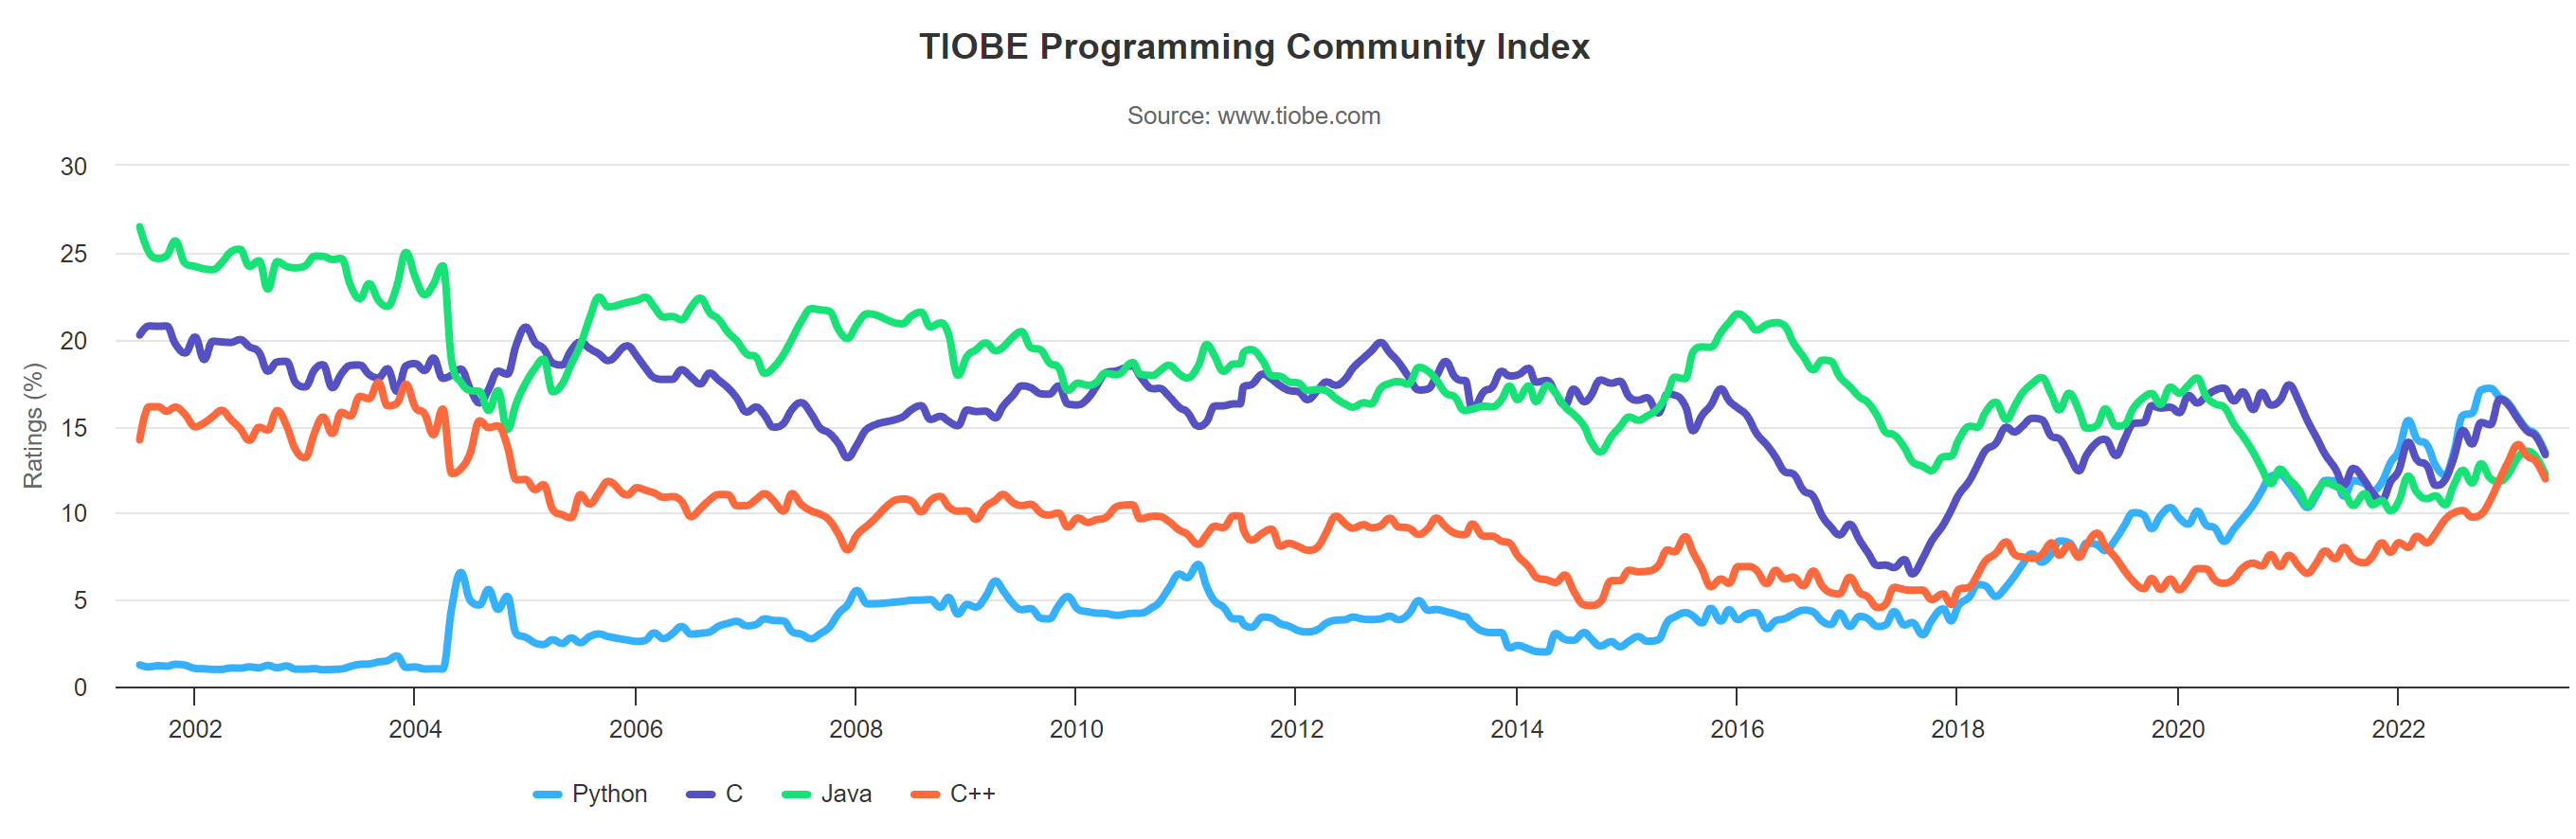
\includegraphics[width=\textwidth]{figures/tiobe.png}
    \caption{主要编程语言流行度变化}
    \label{fig:tiobe}
\end{figure}

Python 具有良好的生态,发展出了丰富的标准库和第三方库,可以满足基本功能开发的需求。Python 的语言特点满足了模块化的需求,有利于对功能的扩展与更新。同时,Python 简洁、方便的语言风格使其可以快速开发性能需求不高的插件。

C++ 拥有很高的效率,使其满足对效率要求较高的插件的开发。同时,Cpython 作为 Python 官方实现,是最广泛使用的解释器之一 \cite{c_py}。得益于此,使用 C++ 编写 Python 模块的技术支持和社区支持都十分完善 \cite{cmodule_py}。

\subsection{经济可行性研究}

本软件的开发有成熟的技术技术,不依赖于特定服务,仅在本地部署,不需要额外投入资金。

\section{需求分析}

\subsection{功能需求}

\begin{enumerate}
    \item 文件信息的查看。对于所有的文件,本软件应分析内容和附加信息,从中提取出有用的部分,当用户或插件需要时,以用户或程序友好的形式呈现给用户或传输给插件。同时,对于所有文件,应当有一个总体的统计分析。
    \item 相似相同文件检索。对于普通文件,本软件应检索出字节码完全相同的文件;对于媒体文件,本软件应额外进行相似文件检索;特别的,对于图像文件,若一个图像是另一个图像的子图(本文中出现的“子图”均指文件类型意义上的图像(image),而不是离散数学意义上的图(graph)),则匹配子图的位置。
    \item 标签管理。对于普通文件,本软件应具备自动给文件添加标签功能,同时留有接口让插件或用户添加、删除标签;对于媒体文件,应进行额外的分析,通过模型或 API ,以及一定的逻辑,添加标签。
    \item 标签检索。对满足特定标签的文件进行检索。
    \item 归类整理。本软件应具备通过文件元信息和标签将文件归类整理的功能。
    \item GUI。本软件应具有一个图形化界面,图形化界面中应能够显示根据文件生成的缩略图。
\end{enumerate}

\subsection{非功能需求}

\begin{enumerate}
    \item 性能需求。在读取和处理媒体文件的过程中,涉及音视频的编码,应保证一定的效率。在自动化过程中,可能需要使用通过机器学习生成的模型,或是连接在线的 API ,需要达到用户无感知的程度。
    \item 鲁棒性需求。用户进行的正常操作不应产生异常;插件产生的异常或效率问题应及时被本软件主体程序处理。
    \item 扩展性需求。开发者应可以方便地编写此软件的插件。
    \item 跨平台需求。本软件应能够在桌面环境和服务器环境中正常运行。
    \item 安全性需求。本软件应降低对用户文件的控制,提高用户文件的安全性。
    \item 开源需求。本软件应遵循依赖项和参考项目的开源许可证,并以不引起冲突的方式发布源代码。
\end{enumerate}

\section{系统架构}

本软件主体部分将只保留必要的逻辑,其中包括插件管理系统。需求分析中出现的其它功能全部以插件的形式实现,包括文件信息查看、相似相同文件检索、标签管理、归类整理、GUI、与数据库通信等功能。本软件的内核将默认附加部分插件。这些插件虽然和本软件的内核在同一个软件包中一并提供,但是并不属于内核。

其中,“以程序友好的形式传输文件信息”功能包含在内核的“必要的逻辑”中,不作为插件单独出现。

\section{插件设计}

本软件的内核将默认附加以下基本插件:

\begin{enumerate}
    \item 文件信息分析插件。在软件主体部分初始化文件时,分析文件的内容和附加信息,并以数据结构的方式储存在内存中。
    \item 标签生成插件。通过文件信息给文件打标签。
    \item 基于多用途互联网邮件扩展(Multipurpose Internet Mail Extensions, MIME)的标签生成插件。通过于互联网号码分配局(Internet Assigned Numbers Authority, IANA)已注册的多用途互联网邮件扩展官方类型数据库以及附加的非标准类型数据库给文件打标签。
\end{enumerate}

上述插件将随软件内核一并提供。

此外,还提供了以下可选插件:

\begin{enumerate}
    \item 单元测试插件。本插件能够以多种方式构造多个测试用例,测试本软件内核和默认附加插件的正确性、鲁棒性和安全性。同时,它可以测试插件的可用性。 % test (to fix)
    \item 文件信息统计插件。此插件能够在全局角度下统计文件信息。 % pie (to fix)
    \item 基于 ANSI 控制符的文件信息查看插件。此插件能够以用户友好的方式显示文件信息。 % show (todo)
    \item 基于多用途互联网邮件扩展的归类整理插件。此插件通过文件多用途互联网邮件扩展的类型将文件归类整理。此插件依赖于基于多用途互联网邮件扩展的标签生成插件。 % destination
    \item 基于 FFmpeg 的媒体文件信息分析插件。此插件通过 FFmpeg 中的命令行工具 ffprobe 分析媒体文件。 % ffprobe (todo)
    \item 基于散列的相同文件检索插件。此插件通过文件的散列值检索完全相同的文件。 % hash
    \item 基于感知散列(Perceptual hashing, pHash)的相似图像检索插件。此插件通过生成图像的指纹并进行比较检索相似图像。 % simimg
    \item 基于分块加速和感知散列的相似图像快速检索插件。此插件通过生成图像的指纹并进行比较检索相似图像,通过分块算法进行加速。此插件是基于感知散列的相似图像检索插件的增强。 % simimg
    \item 基于 PyParsing 的递归下降集合运算解释器插件。此插件能够解析集合运算语句。 % taggy
    \item 基于集合运算解释器的检索插件。通过给出的集合运算语句检索满足相应标签要求的图片。此插件依赖于基于 PyParsing 的递归下降集合运算解释器插件。 % taggy
    \item 基于文件标签的归类整理插件。此插件通过文件元信息和标签将文件归类整理。此插件是基于多用途互联网邮件扩展的归类整理插件的增强,依赖于基于集合运算解释器的检索插件。 % destination
    \item 基于 Flask 的 GUI 插件。此插件为本软件提供图形化界面。此插件可以连接基于集合运算解释器的检索插件和基于文件标签的归类整理插件进行展示。 % flask
    \item 基于粒子群优化(Particle Swarm Optimization, PSO)的子图匹配插件。此插件通过粒子群优化匹配图像的子图。 % rimo (to fix)
    \item 基于 GoogLeNet 的图像标签生成插件。此插件通过 GoogLeNet 学习得到的模型给图像文件打标签。 % ggnet (to fix)
\end{enumerate}

\section{开发环境和运行环境}

本软件开发过程中使用的环境如下:

\begin{enumerate}
    \item 操作系统:Manjaro。
    \item 编辑器:Visual Studio Code,VIM。
    \item C/C++ 编译器:支持 C++ 11 的编译器。
    \item 壳层(Shell):Zsh,Fish。
    \item 中央处理器(Central processing unit, CPU):AMD(Advanced Micro Devices,超微半导体) Ryzen(锐龙) 5950x 16-Core Processor (处理器)。
    \item 图形处理器(Graphics processing unit, GPU):NVIDIA(英伟达) GeForce RTX 3080 Ti(Titanium,钛),支持 CUDA (Compute Unified Device Architecture,统一计算架构)和 CUDNN (Compute Unified Device Architecture Deep Neural Network, CUDA Deep Neural Network,深度神经网络统一计算架构)。
    \item 内存:8 GB 以上。
    \item 硬盘:大于 512 GB 可用空间。
\end{enumerate}

系统运行所需的软件环境为:

\begin{enumerate}
    \item Python 版本:3.7 及以上。
\end{enumerate}

若需要使用可选插件,则可能需要额外安装依赖:

\begin{enumerate}
    \item Flask 版本:2.0 及以上。
    \item TensorFlow 版本:1.19 及以上。
    \item OpenCV(C++ 依赖库)版本:3.4 及以上。
    \item FFmpeg 版本:3.4 及以上。
\end{enumerate}

在软件环境中,平台支持较为全面、安装较为便捷、接口较为稳定的依赖将不额外赘述,如一些常见的开发运行库,Git 等常见的工具,Python 的 OpenCV、NumPy、SciPy、PySwarms、Pillow、Matplotlib 等模块,Linux 中的 GCC 等包。

系统运行所需的最低硬件环境要求为:

\begin{enumerate}
    \item 中央处理器:多核处理器。
    \item 内存:2 GB 以上。
    \item 硬盘:大于 1 GB 可用空间。
\end{enumerate}

上述最低硬件环境要求仅为维持本软件内核的安装和运行所需的最低要求。在以下的建议配置上,可以获得更好的体验:

\begin{enumerate}
    \item 中央处理器:Intel® Core™ i7-4770K、AMD Ryzen 5 1500X 或相似性能的中央处理器及以上。
    \item 内存:4 GB 以上。
    \item 硬盘:大于 16 GB 可用空间。
\end{enumerate}

\section{开源许可证}

经过调查和分析,本软件避免了直接使用以 GPL 许可证发布的代码,避免了调用以 AGPL 许可证发布的软件。

其中,FFmpeg 同时存在两个版本:以 GPL 发布的版本和以 LGPL 发布的版本 \cite{ffmpeg_doc}。本软件使用以 LGPL 发布的版本。
